% !TeX TS-program = xelatex

\documentclass{beamer}
%Set the slide theme
%Change to meet your taste
% Madrid, Copenhagen, Berlin, ... works
\usetheme{metropolis}

\usepackage{multicol}

\usepackage{ragged2e} % who justifies the text
\usepackage{xecolor}
\usepackage{amsmath}
%\usefonttheme[onlymath]{serif} %Change the math font

\usepackage{multirow}
\usepackage{tabularx}
\usepackage{booktabs}
\usepackage[style=numeric]{biblatex}
\addbibresource{references.bib}
\usepackage{xepersian}
\settextfont[Path=fonts/]{Parastoo}

%---------------------------------------------------------------------------------
% Seetings to force Beamer works with Xepersian and RTL typesetting
%-------------------------------------------------------------------------------
%\raggedleft

% For right to left lists (itemize and enumerate)
\makeatletter
\newcommand{\RTList}{\raggedleft\rightskip\@totalleftmargin}
\makeatother
% Correct the bullet for RTL texts
\setbeamertemplate{itemize item}{\scriptsize\raise1.25pt%
 \hbox{\donotcoloroutermaths$\blacktriangleleft$}} 

% To force beamer use numbering in captions
\setbeamertemplate{caption}[numbered]{}% Number float-like environments

\setbeamertemplate{footline}[frame number]
\setbeamertemplate{section in toc}[circle]
\setbeamertemplate{blocks}[rounded][shadow=true]
\setbeamercolor{block body}{bg=lightgray}

\setbeamertemplate{headline}
{
    \begin{beamercolorbox}{section in head/foot}
        \vspace{2pt}\insertnavigation{\paperwidth}\vspace{2pt}
    \end{beamercolorbox}
}

%---------------------------------------------------------------------------------
\title{
    زنجیره‌سازی کارکردهای مجازی سرویس شبکه با در نظر گرفتن محدودیت منابع مدیریتی
}
\subtitle{}
\author{پرهام الوانی}
\institute{
    دانشکده مهندسی کامپیوتر\\دکتر بهادر بخشی
}
\date{شهریور ۱۳۹۸}

\begin{document}
\begin{persian}

\makeatletter
\setbeamertemplate{title page}{
  \begin{minipage}[b][\paperheight]{\textwidth}
    \begin{center}
        \ifx\inserttitlegraphic\@empty\else\usebeamertemplate*{title graphic}\fi
    \end{center}
    \vfill%
    \ifx\inserttitle\@empty\else\usebeamertemplate*{title}\fi
    \ifx\insertsubtitle\@empty\else\usebeamertemplate*{subtitle}\fi
    \usebeamertemplate*{title separator}
    \ifx\beamer@shortauthor\@empty\else\usebeamertemplate*{author}\fi
    \ifx\insertdate\@empty\else\usebeamertemplate*{date}\fi
    \ifx\insertinstitute\@empty\else\usebeamertemplate*{institute}\fi
    \vspace*{5mm}
    \begin{center}
        
\includegraphics[width=1cm]{images/logo}
    \end{center}
    \vfill
    \vspace*{1mm}
  \end{minipage}
}

\setbeamertemplate{title}{
%  \raggedright%  % <-- Comment here
  \linespread{1.0}%
  \inserttitle%
  \par%
  \vspace*{0.5em}
}
\setbeamertemplate{subtitle}{
%  \raggedright%  % <-- Comment here
  \insertsubtitle%
  \par%
  \vspace*{0.5em}
}
\makeatother

%------------------------------------------
% Title frame (0)
%------------------------------------------
\begin{frame}
    \titlepage{}
\end{frame}

% To adjust the paragraphs in RTL
\everypar{\rightskip\rightmargin}
%-------------------------------------------------------------------------------
\begin{frame}{فهرست}
    \tableofcontents
\end{frame}
%-------------------------------------------------------------------------------
\begin{frame}{}
    \section{مقدمه}
\end{frame}
%-------------------------------------------------------------------------------
\begin{frame}{شبکه‌های سنتی}
    \begin{itemize}\RTList{}
        \justifying
        \item یک سرویس شبکه به صورت تعدادی کارکرد مشخص که ترافیک با ترتیب مشخصی از آن ها عبور می‌کند، تعریف می‌شود.
        \item کارکردهای شبکه به صورت سخت‌افزار و نرم‌افزار اختصاصی تهیه شده از سازندگان مختلف استفاده می‌شوند.
        \item کارکردها باید در مکان مناسب در شبکه قرار گیرند و ترافیک به سمت آن‌ها هدایت شود.
    \end{itemize}
\end{frame}
%-------------------------------------------------------------------------------
\begin{frame}{شبکه های سنتی}
    \begin{itemize}\RTList{}
        \justifying
        \item افزایش نیازمندی به سرویس‌های متنوع با عمرکوتاه و نرخ بالای ترافیک
        \begin{itemize}\RTList{}
            \item خریداری، انبارداری و استقرار سخت‌افزارهای اختصاصی
            \item افزایش هزینه‌های خرید، آموزش و انبارداری
            \item کاهش فضای فیزیکی
            \item سربار آموزش کارکنان
            \item محدودیت نوآوری در سخت‌افزار و سرویس
        \end{itemize}
    \end{itemize}
    \begin{block}{}
        \centering
        \lr{Network Functions Virtualization}\\
        مجازی‌سازی کارکردهای شبکه
    \end{block}
\end{frame}
%-------------------------------------------------------------------------------
\begin{frame}{شبکه های سنتی}
    \begin{itemize}\RTList{}
        \justifying
        \item ترافیک کاربر باید از تعدادی کارکرد شبکه به ترتیب معینی عبور کند.
        \item کارکردها به صورت سخت‌افزاری به یکدیگر متصلند و ترافیک با استفاده از جداول مسیریابی به سمت آن‌ها هدایت می شود.
        \item نیاز به تغییر همبندی سریع و یا مکان کارکردها برای سرویس‌دهی بهتر 
        \begin{itemize}\RTList{}
            \item استقرار و تغییر ترتیب کارکردها دشوار است
            \item امکان رخدادن خطاهای متعدد
        \end{itemize}
    \end{itemize}
    \begin{block}{}
        \centering
        \lr{Service Function Chaining}\\
        زنجیره‌سازی کارکرد سرویس
    \end{block}
\end{frame}
%-------------------------------------------------------------------------------
\begin{frame}{معماری پیشنهادی}
    \begin{itemize}\RTList{}
        \justifying
        \item مجازی‌سازی کارکردهای شبکه 
        \begin{itemize}\RTList{}
            \item اواخر سال ۲۰۱۲، \lr{ETSI NFV ISG} توسط هفت اپراتور جهانی شبکه تأسیس شد.
            \item اکنون بیش از 250 سازمان با آن همکاری می‌کنند.
            \item اجرای کارکردها بر روی سرورهای استاندارد با توان بالا به وسیله مجازی‌سازی کارکردها
            \begin{itemize}\RTList{}
                \item کاهش نیاز به تجهیزات سخت‌افزاری خاص منظوره
                \item اشتراک گذاری منابع بین کارکرد‌ها
                \item کاهش هزینه‌های تجهیزات و مصرف انرژی از طریق تجمیع کارکردها
            \end{itemize}
        \end{itemize}
        \item زنجیره‌سازی کارکرد سرویس
        \begin{itemize}\RTList{}
            \item امکان تعریف زنجیره کارکردها به صورت پویا و بدون تغییر در زیرساخت فیزیکی
            \item \lr{RFC 7665}
        \end{itemize}
    \end{itemize}
\end{frame}
%-------------------------------------------------------------------------------
\begin{frame}{معماری پیشنهادی}
    \begin{center}\begin{figure}
        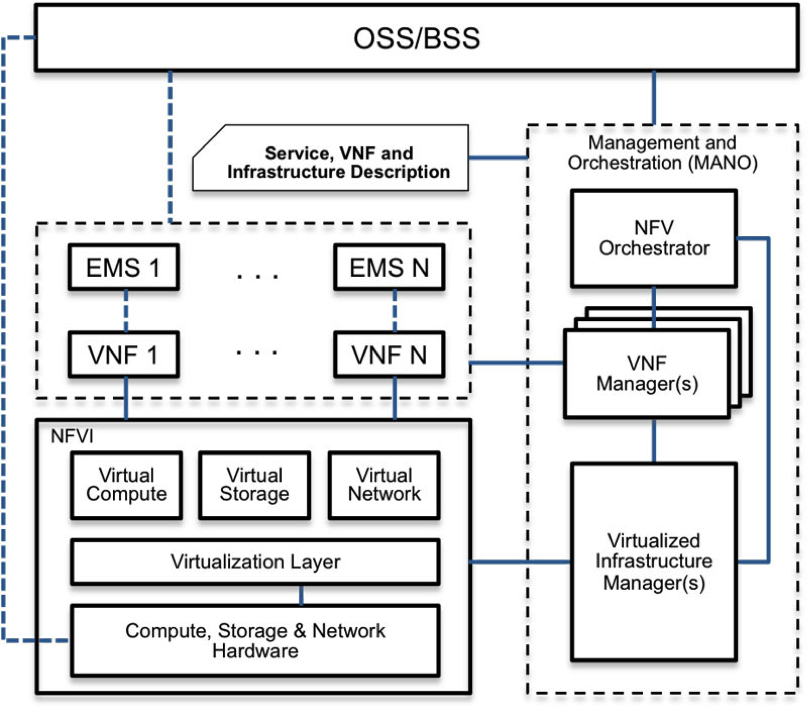
\includegraphics[scale=0.5]{images/nfv-arch.png}
        \caption{معماری سطح بالای مجازی‌سازی کارکردهای شبکه}
    \end{figure}\end{center}
\end{frame}
%-------------------------------------------------------------------------------
\begin{frame}{مقدمه}
    \begin{itemize}\RTList{}
        \item \lr{NFVO} وظیفه‌ی استقرار زنجیره‌های کارکرد سرویس را برعهده دارد.
        \item \lr{VNFM} مسئول چرخه‌ی زندگی کارکردهای مجازی شبکه می‌باشد.
        \item چرخه‌ی زندگی هر کارکرد مجازی شامل عملیات‌هایی همچون نمونه‌سازی، مقیاس‌کردن، به‌روزرسانی و پایان دادن می‌باشد.
        \item هر نمونه از کارکردهای مجازی شبکه نیاز دارد تحت مدیریت یکی از \lr{VNFM}های موجود در شبکه باشد.
    \end{itemize}
\end{frame}
%-------------------------------------------------------------------------------
\begin{frame}{چالش‌ها}
    \begin{columns}
        \begin{column}{0.6\textwidth}
            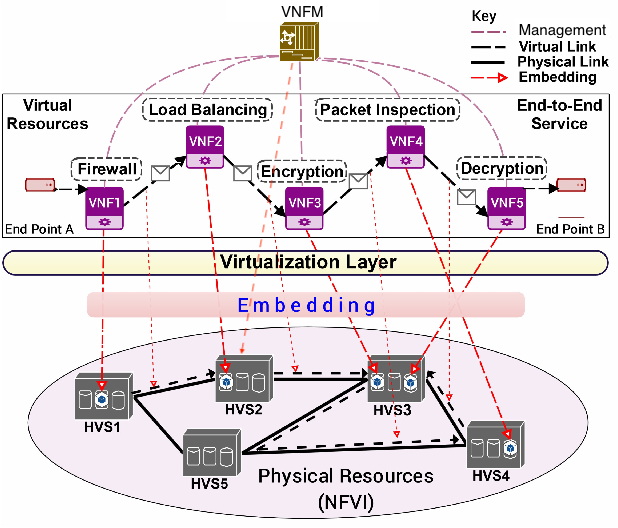
\includegraphics[scale=0.35]{images/embedding.png}
        \end{column}
        \begin{column}{0.4\textwidth}
            \begin{itemize}\RTList{}
                \item مدیریت و هماهنگی
                \item مصرف بهینه‌ی انرژی
                \item تخصیص منابع به کارکردهای مجازی
                \item مسیریابی زنجیره‌های کارکرد سرویس
                \item پذیرش زنجیره‌های کارکرد سرویس
                \item به روزرسانی و مقیاس کردن کارکردهای مجازی سرویس
            \end{itemize}
        \end{column}
    \end{columns}
\end{frame}
%-------------------------------------------------------------------------------
\begin{frame}{}
    \section{سابقه‌ی کارها}
\end{frame}
%-------------------------------------------------------------------------------
\begin{frame}{سابقه‌ی کارها}
    \fontsize{6pt}{7.2}\selectfont
    \begin{table}[h]
        \caption{مقایسه مقالات پذیرش زنجیره‌های کارکرد سرویس}
        \vspace{0.5cm}
        \begin{tabularx}{\textwidth}{XXXXXXXXXXXXXXXXX}
            \toprule
            منبع &
            \multicolumn{4}{X}{منابع تخصیص یافته} &
            \multicolumn{2}{X}{محدودیت ظرفیت پردازشی نمونه} &
            \multicolumn{2}{X}{برخط یا برون خط} &
            \multicolumn{2}{X}{نگاشت کارکرد و لینک} &
            \multicolumn{2}{X}{انتساب کارکرد} &
            \multicolumn{2}{X}{اشتراک نمونه} &
            \multicolumn{2}{X}{تخصیص \lr{VNFM}} \\
            \midrule
            \lr{\#} &
            \lr{other} &
            \lr{MEM} &
            \lr{BW} &
            \lr{CPU} &
            دارد &
            ندارد &
            برخط &
            برون خط &
            کارکرد &
            لینک &
            یک نمونه &
            چند نمونه &
            دارد &
            ندارد &
            دارد &
            ندارد \\
            \midrule
            \cite{Eramo2016} &
            \lr{---} &
            \lr{---} &
            \checkmark&
            \checkmark&
            \lr{---}&
            \checkmark&
            \lr{---} &
            \checkmark&
            \checkmark&
            \checkmark&
            \checkmark&
            \lr{---} &
            \lr{---} &
            \checkmark&
            \lr{---} &
            \checkmark\\
            \midrule
            \cite{Ghaznavi2017} &
            \lr{---} &
            \lr{---} &
            \checkmark&
            \checkmark&
            \checkmark&
            \lr{---} &
            \lr{---} &
            \checkmark&
            \checkmark&
            \checkmark&
            \lr{---} &
            \checkmark&
            \lr{---} &
            \checkmark&
            \lr{---} &
            \checkmark\\
            \midrule
            \cite{Huang2017} &
            \lr{---} &
            \lr{---} &
            \checkmark&
            \checkmark&
            \checkmark&
            \lr{---} &
            \lr{---} &
            \checkmark&
            \checkmark&
            \checkmark&
            \lr{---} &
            \checkmark&
            \lr{---} &
            \checkmark&
            \lr{---} &
            \checkmark\\
            \midrule
            \cite{AbuLebdeh2017} &
            \lr{VNFM capacity} &
            \lr{---} &
            \lr{---} &
            \lr{---} &
            \lr{---} &
            \checkmark&
            \checkmark&
            \lr{---} &
            \lr{---} &
            \checkmark &
            \lr{---} &
            \lr{---} &
            \lr{---} &
            \lr{---} &
            \checkmark&
            \lr{---} \\
            \midrule
            پژوهش حاضر &
            \lr{---} &
            \checkmark&
            \checkmark&
            \checkmark&
            \checkmark&
            \lr{---} &
            \lr{---} &
            \checkmark&
            \checkmark&
            \checkmark&
            \checkmark&
            \lr{---}&
            \lr{---}&
            \checkmark&
            \checkmark&
            \lr{---}\\
            \bottomrule
        \end{tabularx}
    \end{table}
\end{frame}
%-------------------------------------------------------------------------------
\begin{frame}{سابقه‌ی کارها}
    \begin{itemize}\RTList{}
        \item این مقاله مساله‌ی جایگذاری \lr{VNFM}ها را مطرح می‌کند.
        \item این مقاله فرض می‌کند زنجیره‌های جایگذاری شده‌اند و هر در بازه‌ی زمانی می‌توانند بازنگاشت شوند.
        \item این مساله قصد دارد با در نظر گرفتن هزینه‌های عملیاتی مساله‌ی بازنگاشت \lr{VNFM}ها در بازه‌های زمانی را حل کند.
    \end{itemize}
    \begin{latin}
    \fullcite{AbuLebdeh2017}
    \end{latin}
\end{frame}
%-------------------------------------------------------------------------------
\begin{frame}{}
    \section{تعریف مساله}
\end{frame}
%-------------------------------------------------------------------------------
\begin{frame}{تعریف مساله}
    \par
    بیشینه‌سازی سود حاصل از پذیرش زنجیره‌های کارکرد سرویس با در نظر گرفتن کارکرد سرویس با در نظر گرفتن نیاز برخی از نمونه‌های کارکرد
    مجازی شبکه به \lr{VNFM}.
\end{frame}‌
%-------------------------------------------------------------------------------
\begin{frame}{تعریف مساله}
    \begin{itemize}\RTList{}
        \justifying
        \item توپولوژی زیرساخت شامل پنهای باند لینک‌ها و ظرفیت \lr{NFVI-PoP}ها، موجود است.
        \item n تقاضای زنجیره‌ کارکرد سرویس به صورت کامل و از پیش مشخص شده داریم.
        \item هر تقاضا شامل نوع و تعداد نمونه‌های مجازی، پنهای باند لینک‌های مجازی و توپولوژی
        نمونه‌های مجازی می‌باشد.
    \end{itemize}
\end{frame}
%-------------------------------------------------------------------------------
\begin{frame}{تعریف مساله}
    \justifying
    \begin{itemize}\RTList{}
        \item نمونه‌ها بین زنجیره‌ها به اشتراک گذاشته نمی‌شوند.
        \item محدودیت ظرفیت لینک‌ها
        \item محدودیت توان پردازش سرورهای فیزیکی با توجه به میزان حافظه و تعداد پردازنده‌ها
        \item برخی از سرور‌های فیزیکی نمی‌توانند سرور‌های فیزیکی مشخصی را مدیریت کنند.
        \item برخی از سرورهای فیزیکی توانایی پشتیبانی از کارکردهای مجازی را ندارد.
        \item برخی از نمونه‌های کارکرد مجازی تنها می‌توانند روی سرورهایی خاص نگاشته شوند.
    \end{itemize}
\end{frame}
%-------------------------------------------------------------------------------
\begin{frame}{تعریف مساله}
    \justifying
    \begin{itemize}\RTList{}
        \item برای مدیریت یکدست و آسان‌تر زنجیره‌ها و در عین حال جمع‌آوری راحتر خطاها، برای هر زنجیره یک \lr{VNFM} تخصیص می‌دهیم.
        \item \lr{VNFM}ها می‌توانند بین زنجیره به اشتراک گذاشته شوند.
        \item هر نمونه از \lr{VNFM}ها می‌تواند تعداد مشخصی از نمونه‌های کارکرد مجازی شبکه را سرویس دهد. 
        \item برای ارتباط میان هر نمونه از \lr{VNFM}ها و \lr{VNF}ها پهنای باند مشخصی رزرو می‌گردد.
        \item در صورتی که \lr{NFVI-PoP} بتواند از \lr{VNFM} پشتیبانی نماید،
        می‌توان به هر تعداد که ظرفیت آن اجازه می‌دهد بر روی آن \lr{VNFM} نصب نمود.
    \end{itemize}
\end{frame}
%-------------------------------------------------------------------------------
\begin{frame}{چالش‌ها و نوآوری‌های مساله}
    \begin{itemize}\RTList{}
        \item در نظر گرفتن نیازمندی نمونه‌های کارکرد مجازی به یک \lr{VNFM}
        \item در نظر گرفتن نیازمندی تاخیر برای لینک‌های مدیریتی
        \item تخصیص منابع مدیریتی به زنجیره‌ها و مسیریابی ارتباط مدیریتی
        \item جایگذاری و مسیریابی توامان زنجیره‌های کارکرد سرویس
        \item طراحی مساله‌ی نزدیک به واقعیت
    \end{itemize}
\end{frame}
%-------------------------------------------------------------------------------
\begin{frame}{معیار و نحوه‌ی ارزیابی}
    \begin{itemize}\RTList{}
        \item مدل‌سازی مساله
        \item حل مساله‌ی بهینه در ابعاد کوچک
        \item پیاده‌سازی راه‌حل مکاشفه‌ای
        \item معیار مقایسه این راه حل سود حاصل از پذیرش تقاضاهای زنجیره‌های کارکرد سرویس می‌باشد.
        \item مقایسه‌ی نتایج راه‌حل مکاشفه‌ای با جواب بهینه
    \end{itemize}
\end{frame}
%-------------------------------------------------------------------------------
\begin{frame}{}
    \section{فرمول‌بندی و مدل‌سازی ریاضی مساله}
\end{frame}
%-------------------------------------------------------------------------------
\begin{frame}{فرمول‌بندی}
    \par
    هدف اصلی مساله پذیریش بیشترین تعداد تقاضا می‌باشد.
    در اینجا فرض می‌کنیم پذیرش هر تقاضا سودی منحصر به فرد و هزینه‌ای برای تهیه گواهی \lr{VNFM} در بر خواهد داشت.
    بنابراین تابع هدف به شکل زیر می‌باشد:

    \begin{latin}\begin{align}
        max \sum_{h=1}^{T} c_hx_h - \sum_{w \in V_s^{PN}} licenseFee . \bar{y}_w
    \end{align}\end{latin}
\end{frame}
%-------------------------------------------------------------------------------
\begin{frame}{فرمول‌بندی}
    \par
    محدودیت حافظه نودها
    \begin{latin}\begin{align}
        \sum_{k=1}^F y_{wk} memory(k) + \bar{y_w} \bar{memory} \le N_{ram}^{PN}(w)
        \quad
        \forall w \in V_s^{PN}
    \end{align}\end{latin}
    \par
    محدودیت تعداد پردازنده‌های نودها
    \begin{latin}\begin{align}
        \sum_{k=1}^F y_{wk} core(k) + \bar{y_w} \bar{core} \le N_{core}^{PN}(w)
        \quad
        \forall w \in V_s^{PN}
    \end{align}\end{latin}
\end{frame}
%-------------------------------------------------------------------------------
\begin{frame}{فرمول‌بندی}
    \par
    اگر تقاضای \lr{h}ام پذیرفته شده باشد
    می‌بایست تمام \lr{VNF node}های آن‌
    سرویس شده باشند.
    یک \lr{VNF} حداکثر یکبار سرویس داده شود.
    \begin{latin}\begin{align}
        x_h = \sum_{k=1}^{F} \sum_{w \in V_{s}^{PN}} z_{vw}^{k}
        \quad
        \forall v \in V_{h,F}^{SFC}, \forall h \in [1,\ldots, T]
    \end{align}\end{latin}
\end{frame}
%-------------------------------------------------------------------------------
\begin{frame}{فرمول‌بندی}
    \par
    اگر تقاضای \lr{h}ام پذیرفته شده باشد
    می‌بایست توسط یک \lr{VNFM} سرویس شده باشد.
    توجه شود که این محدودیت اجازه‌ی تخصیص بیش از یک \lr{VNFM}
    به زنجیره نمی‌دهد.
    \begin{latin}\begin{align}
        x_h = \sum_{w \in V_{s}^{PN}} \bar{z}_{hw}
        \quad
        \forall h \in [1,\ldots, T]
    \end{align}\end{latin}
\end{frame}
%-------------------------------------------------------------------------------
\begin{frame}{فرمول‌بندی}
    \par
    محدودیت ظرفیت سرویس‌دهی \lr{VNFM}
    این محدودیت براساس تعداد ماشین‌های مجازی که هر
    \lr{VNFM}
    سرویس می‌دهد تعیین شده است.
    در نظر داشته باشید که ممکن است برخی از انواع
    \lr{VNF}‌ها
    نیازی به مدیریت شدن نداشته باشند.

    \begin{latin}
        \begin{align}
            \sum_{i=1}^{T} \bar{z}_{iw} . (len(i) - \sum_{v \in V_{i, F}^{SFC}} \sum_{k \in [1, \dots, F]} type(v, k) . isManageable(k)) \le \nonumber \\
            capacity . \bar{y}_{w}
            \quad
            \forall w \in V_{s}^{PN}
        \end{align}
    \end{latin}
\end{frame}
%-------------------------------------------------------------------------------
\begin{frame}{فرمول‌بندی}
    \par
    اگر \lr{VNF}، \lr{v}
    توسط نمونه‌ای نوع \lr{k}
    روی سرور \lr{w} سرویس می‌شود می‌بایست
    این \lr{VNF} از نوع \lr{k}ام باشد.
    \begin{latin}\begin{align}
        z_{vw}^{k} \le type(v, k)
        \quad
        \forall w \in V_{s}^{PN},
        \forall k \in [1,\ldots, F],
        \forall v \in \cup_{i=1}^T V_{i, F}^{SFC}
    \end{align}\end{latin}
\end{frame}
%-------------------------------------------------------------------------------
\begin{frame}{فرمول‌بندی}
    \par
    در صورتی که سرور \lr{w}
    توانایی اجرای نمونه‌های \lr{VNF}
    را نداشته باشد نباید نمونه‌ای روی آن قرار گیرد.

    \begin{latin}
        \begin{align}
            \sum_{k \in [1, \dots, F]} y_{wk} \le M . vnfSupport(w)
            \quad
            w \in V_{s}^{PN}
        \end{align}
    \end{latin}
\end{frame}
%-------------------------------------------------------------------------------
\begin{frame}{فرمول‌بندی}
    \par
    برخی از سرورهای نمی‌توانند توسط سرورهای مشخصی مدیریت شوند.
    این ویژگی به ادمین شبکه امکان مدیریت بیشتری می‌دهد و او می‌تواند با دست باز تمامی
    سیاست‌های مورد نظرش را اعمال نماید.

    \begin{latin}
        \begin{align}
            1 - z_{vw_1}^k + \bar{z}_{hw_2} = 0
            \quad
            & \forall w_1 \in V_s^{PN} \forall w_2 \in V_s^{PN} \nonumber \\
            & notManagableBy(w_1, w_2) = 1 \nonumber \\
            & \forall h \in [1,\dots,T],
            \forall v \in V_{h,F}^{SFC},
            \forall k \in [1,\dots,T]
        \end{align}
    \end{latin}
\end{frame}
%-------------------------------------------------------------------------------
\begin{frame}{فرمول‌بندی}
    \par
    \lr{Flow Conservation}
    \begin{latin}\begin{align}
        \sum_{(i,j) \in E^{PN}} \tau_{ij}^{(u,v)} - \sum_{(j,i) \in E^{PN}} \tau_{ji}^{(u,v)} = \sum_{k=1}^{F} z_{ui}^{k} - \sum_{k=1}^{F} z_{vi}^{k} \nonumber \\
        \forall i \in V_{S}^{PN}, (u,v) \in E_{h}^{SFC}, h \in [1,\ldots, T]
    \end{align}\end{latin}
\end{frame}
%-------------------------------------------------------------------------------
\begin{frame}{فرمول‌بندی}
    \par
    \lr{Flow Conservation}
    \begin{latin}\begin{align}
        \sum_{(i,j) \in E^{PN}} \bar{\tau}_{ij}^{v} - \sum_{(j,i) \in E^{PN}} \bar{\tau}_{ji}^{v} = \sum_{k=1}^{F} z_{vi}^{k} - \bar{z}_{hi} \nonumber \\
        \forall i \in V_{S}^{PN}, v \in V_{h, F}^{SFC}, h \in [1,\ldots, T]
    \end{align}\end{latin}
\end{frame}
%-------------------------------------------------------------------------------
\begin{frame}{فرمول‌بندی}
    \par
    محدودیت ظرفیت لینک‌ها
    \begin{latin}\begin{align}
        \sum_{v \in \cup_{i=1}^{T} V_{i,F}^{SFC}} \bar{\tau}_{ij}^{v} * \bar{bandwidth} + \sum_{(u,v) \in \cup_{i=1}^{T} E_{i}^{SFC}} \tau_{ij}^{(u,v)} * bandwidth(u,v) \le C_{ij} \nonumber \\
        \forall (i, j) \in E^{PN}
    \end{align}\end{latin}
\end{frame}
%-------------------------------------------------------------------------------
\begin{frame}{فرمول‌بندی}
    \par
    شعاع همسایگی تضمین می‌کند که زمان سرویس‌دهی توسط
    \lr{VNFM}ها
    در یک بازه مشخص (از نظر تعداد گام)
    خواهد بود.
    \begin{latin}\begin{align}
        \sum_{(i, j) \in E^{PN}} \bar{\tau}_{ij}^{v} \le radius
        \quad
        \forall v \in \cup_{i=1}^T V_{i, F}^{SFC}
    \end{align}\end{latin}
\end{frame}
%-------------------------------------------------------------------------------
\begin{frame}{مساله‌ی نمونه}
    \par
    زنجیره‌های زیر را به عنوان تقاضاها در نظر می‌گیریم.

    \begin{center}
        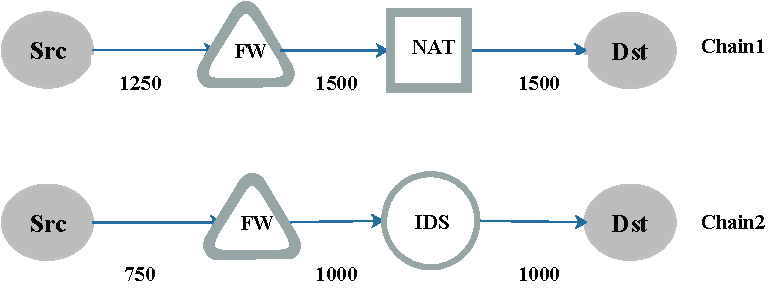
\includegraphics[scale=0.5]{../diagrams/chains.pdf}
    \end{center}
\end{frame}
%-------------------------------------------------------------------------------
\begin{frame}{مساله‌ی نمونه}
    \par
    فرض می‌کنیم مرکز داده‌ای دارای توپولوژی زیر می‌باشد.

    \begin{center}
        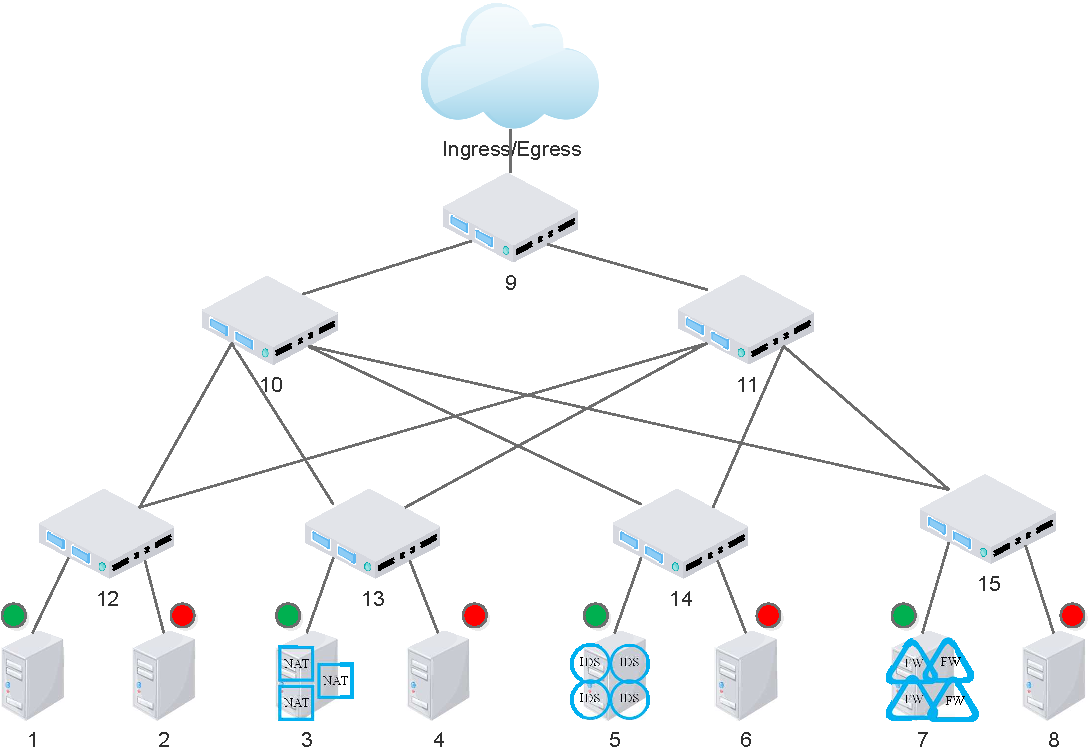
\includegraphics[scale=0.4]{../diagrams/topology.pdf}
    \end{center}
\end{frame}
%-------------------------------------------------------------------------------
\begin{frame}{مساله‌ی نمونه}
    \begin{table}[h]
        \caption{نیازمندی نمونه‌های مساله‌ی نمونه}
        \vspace{0.5cm}
        \begin{center}\begin{latin}\begin{tabular}{|c|c|c|c|}
            \hline
            Spec/VNF & vFW & vNAT & vIDS \\
            \hline
            CPU (vCore) & 2 & 2 & 2 \\
            \hline
            Memory (GB) & 2 & 4 & 2 \\
            \hline
        \end{tabular}\end{latin}\end{center}
    \end{table}
\end{frame}
%-------------------------------------------------------------------------------
\begin{frame}{مساله‌ی نمونه}
    \begin{figure}[h!]
        \caption{مشخصات سرورهای زیرساخت مساله‌ی نمونه}
        \vspace{0.5cm}
        \begin{center}\begin{latin}\begin{tabular}{|c|c|c|}
            \hline
            & Server 1,2,7,8 & Servers 3,4,5,6 \\
            \hline
            Installed vCPU & 144 & 72 \\
            \hline
            Installed Memory (GB) & 1408 & 288 \\
            \hline
            Link (Gbps) & 40 & 40 \\
            \hline
        \end{tabular}\end{latin}\end{center}
    \end{figure}
\end{frame}
%-------------------------------------------------------------------------------
\begin{frame}{مساله‌ی نمونه}
    \begin{itemize}\RTList{}
        \item نمونه‌ها تنها می‌توانند روی سرورهای ۱، ۳، ۵ و ۷ قرار گیرند.
        \item مدیریت سرورهای ۱ و ۳ تنها می‌تواند روی سرورهای ۲ و ۴  صورت گیرد،
        \item مدیریت سرور ۵ تنها می‌تواند روی سرورهای ۴ و ۶ صورت گیرد.
        \item مدیریت سرور ۷ تنها می‌تواند روی سرورهای ۶ و ۸ صورت گیرد.
    \end{itemize}
\end{frame}
%-------------------------------------------------------------------------------
\begin{frame}{مساله‌ی نمونه}
    \begin{itemize}\RTList{}
        \item هر \lr{VNFM} تنها می‌تواند ۵ نمونه را پشتیبانی کند.
        \item هر \lr{VNFM} نیاز به ۴ گیگابایت حافظه و ۲ هسته‌ی پردازشی دارد.
    \end{itemize}
\end{frame}
%-------------------------------------------------------------------------------
\begin{frame}{مساله‌ی نمونه}
    \begin{table}[h!]
        \caption{نتایج مساله‌ی نمونه}
        \vspace{0.5cm}
        \begin{center}\begin{latin}\begin{tabular}{|c|c|c|c|c|c|}
            \hline
            & Src & Node-0 & Node-1 & Dst & VNFM \\
            \hline
            Chain 0 & Switch-9 & Server-7 & Server-5 & Switch-9 & Server-6 \\
            \hline
            Chain 1 & Switch-9 & Server-3 & Server-3 & Switch-9 & Server-4 \\
            \hline
        \end{tabular}\end{latin}\end{center}
    \end{table}
\end{frame}
%-------------------------------------------------------------------------------
\begin{frame}{}
    \section{راه‌حل پیشنهادی}
\end{frame}
%-------------------------------------------------------------------------------
\begin{frame}{راه‌حل پیشنهادی}
    \begin{itemize}\RTList{}
        \item مساله‌ی اصلی یک مساله‌ی \lr{NP-Hard} می‌باشد.
        \item برای حل مساله در زمان معقول برای ابعاد بزرگ نیاز به یک الگوریتم مکاشفه‌ای می‌باشد.
        \item از ایده‌ی الگوریتم \lr{\cite{Bari2015}} برای جایگذاری زنجیره‌ها شروع می‌کنیم.
    \end{itemize}
\end{frame}
%-------------------------------------------------------------------------------
\begin{frame}{ایده‌ی اصلی}
    \begin{center}
        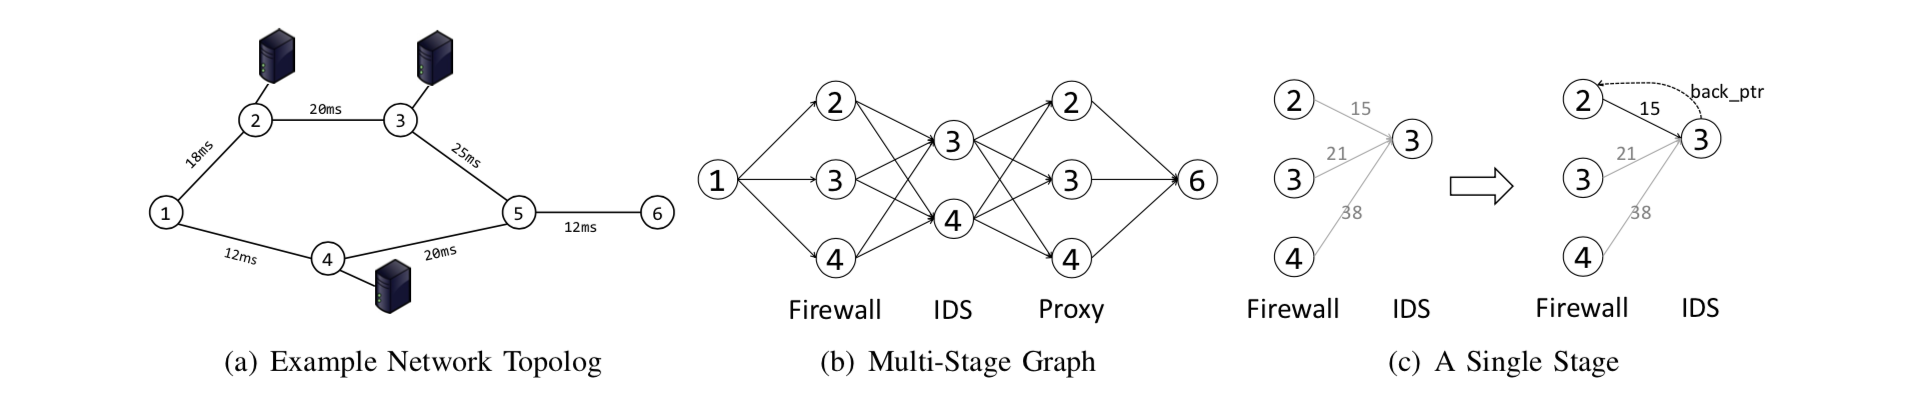
\includegraphics[scale=0.3]{images/bari.png}
    \end{center}
    \begin{itemize}\RTList{}
        \item الگوریتم برای جایگذاری زنجیره از یک گراف چند مرحله‌ای استفاده می‌کند.
        \item در هر مرحله جایگذاری مرحله‌ی قبلی نهایی می‌شود و بر اساس آن یک مجموعه‌ی امکان‌پذیر شکل می‌گیرد.
    \end{itemize}
\end{frame}
%-------------------------------------------------------------------------------
\begin{frame}{\lr{JSD-MP}}
    \begin{itemize}\RTList{}
        \item \lr{Joint Service Deployment - Manager Placement}
        \item زنجیره‌ها را با استفاده از الگوریتم \lr{\cite{Bari2015}} جایگذاری می‌کنیم.
        \item در زمان انتخاب مجموعه‌ی امکان‌پذیر محدودیت‌های مساله را اعمال می‌کنیم.
        \item بعد از جایگذاری هر زنجیره \lr{VNFM} آن را انتخاب می‌کنیم.
        \item برای انتخاب \lr{VNFM} اولویت با نمونه‌هایی است که ظرفیت آن‌ها کامل استفاده نشده است.
        \item در بین \lr{VNFM}هایی که ظرفیت خالی دارند اولویت با نمونه‌هایی است که منابع پردازشی بیشتری دارند.
    \end{itemize}
\end{frame}
%-------------------------------------------------------------------------------
\begin{frame}{\lr{eJSD-MP}}
    \begin{itemize}\RTList{}
        \item الگوریتم پیشنهادی \lr{JSD-MP} زمان اجرای زیادی دارد که می‌توان آن را کاهش داد.
        \item الگوریتم پیشنهادی \lr{eJSD-MP} از برون‌خط بودن مساله استفاده نمی‌کند.
        \item برای استفاده از ویژگی برون‌خط بودن مساله زنجیره‌ها را بر اساس قیمت‌شان مرتب می‌کنیم.
        \item برای کاهش زمان اجرای الگوریتم نسب مشخصی از زنجیره‌ها را با الگوریتم \lr{first-fit} جایگذاری می‌کنیم.
        \item \lr{enhanced JSD-MP}
    \end{itemize}
\end{frame}
%-------------------------------------------------------------------------------
\begin{frame}{}
    \section{ارزیابی}
\end{frame}
%-------------------------------------------------------------------------------
\begin{frame}{پیاده‌سازی بهینه}
    \par
    فرمول‌بندی ارائه شده بر روی نرم‌افزار
    \lr{CPLEX}
    که محصول شرکت \lr{IBM} بوده و برای حل مسائل برنامه‌ریزی خطی و ...
    استفاده می‌شود،
    به زبان جاوا پیاده‌سازی شده است.

    \begin{center}
        
\includegraphics[scale=0.4]{images/ibm-cplex.png}
    \end{center}
\end{frame}
%-------------------------------------------------------------------------------
\begin{frame}{توپولوژی \lr{FatTree}}
    \begin{center}
        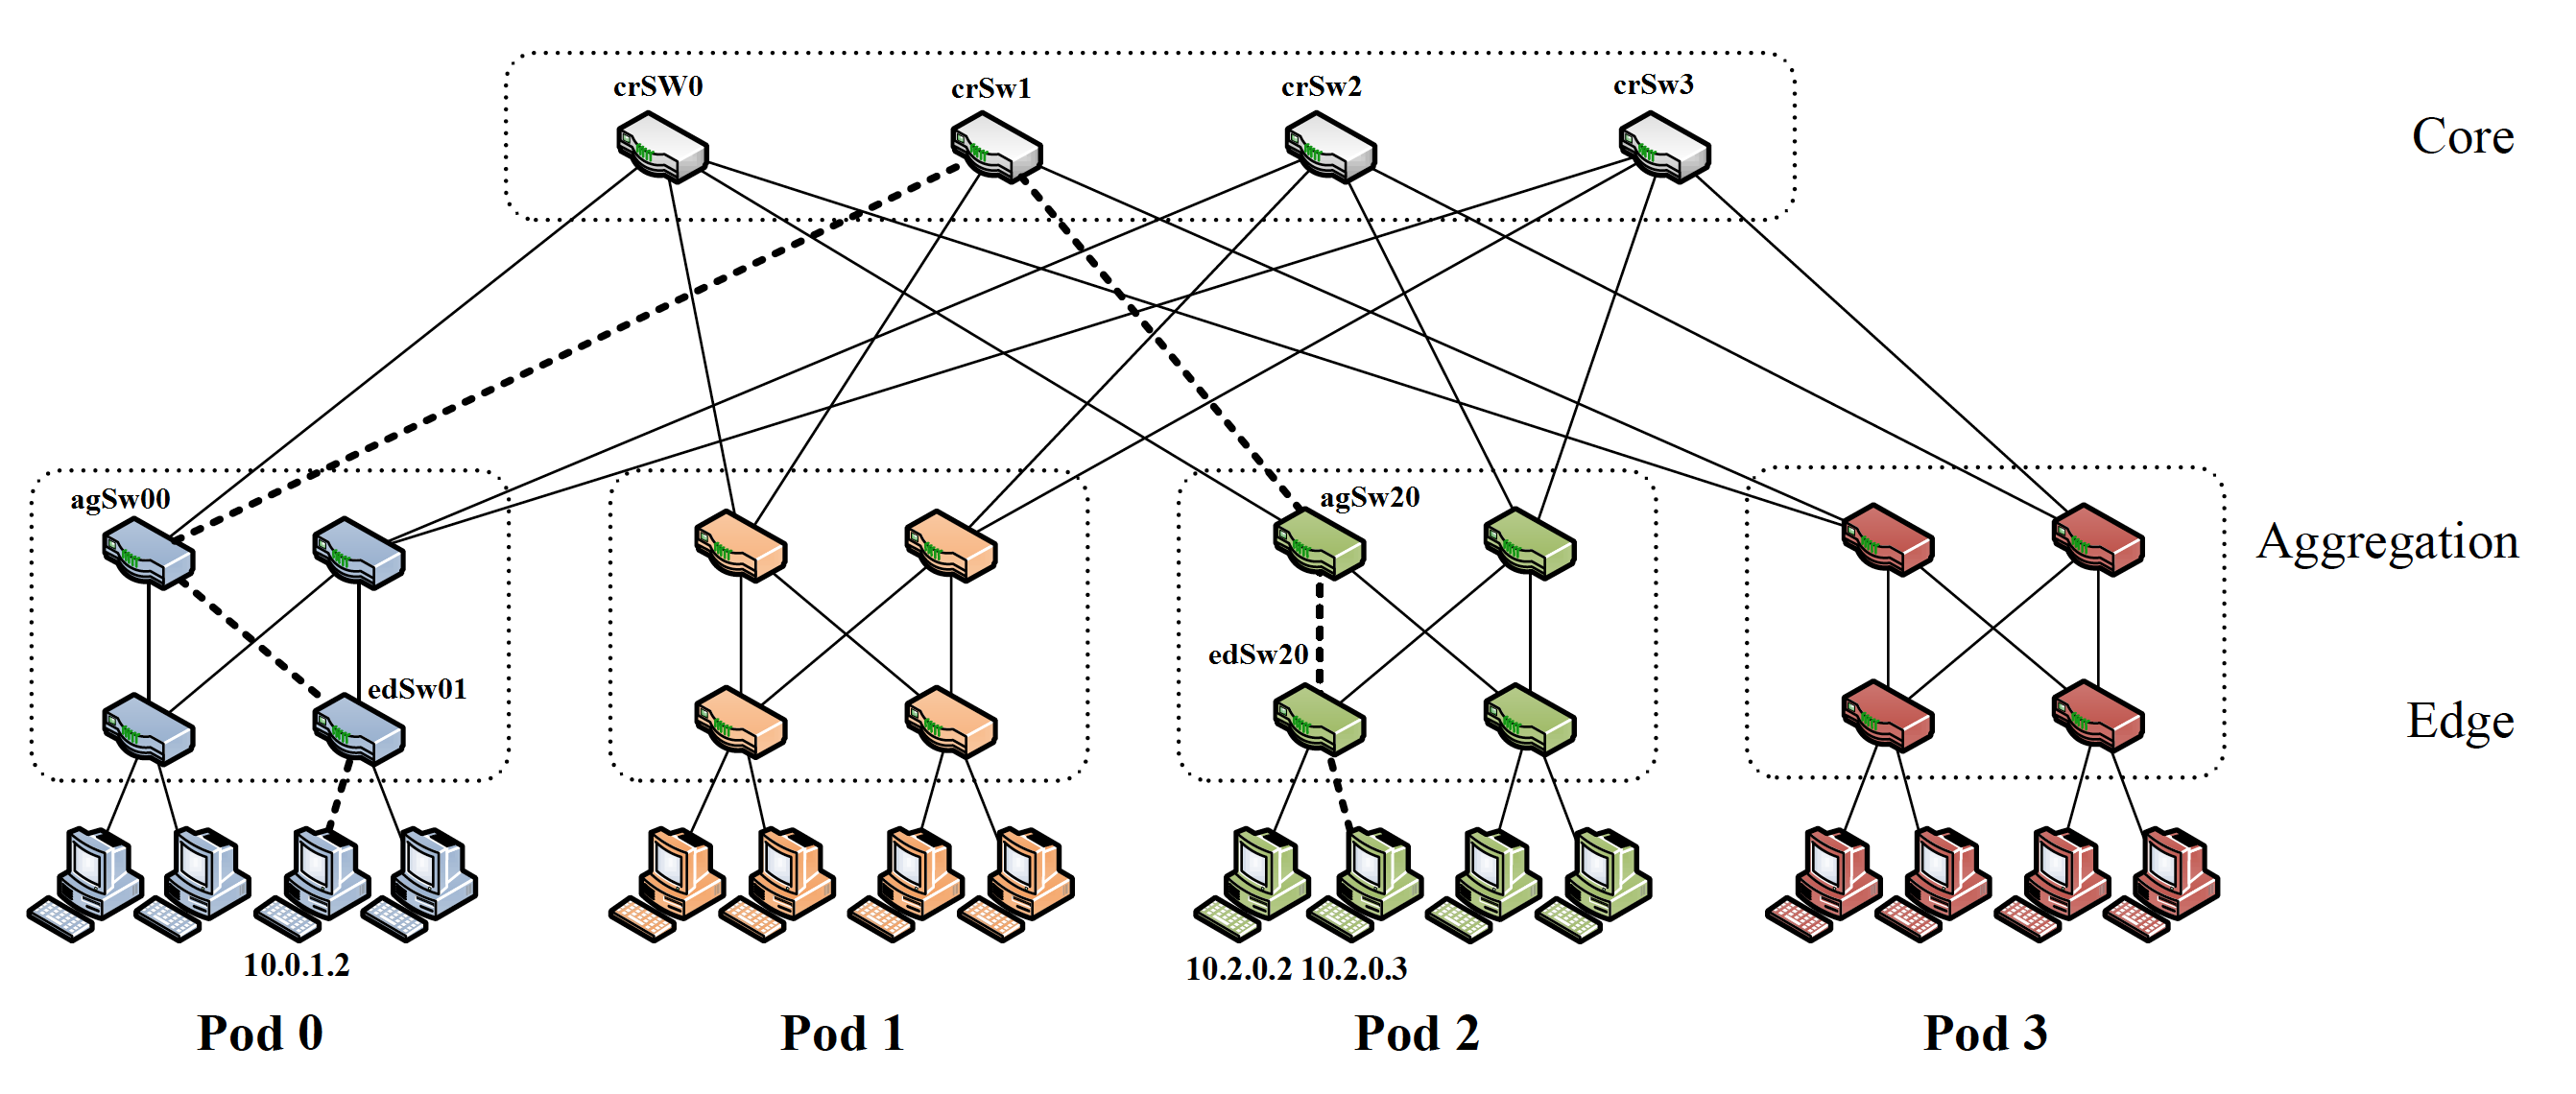
\includegraphics[scale=0.15]{images/fattree.png}
    \end{center}
\end{frame}
%-------------------------------------------------------------------------------
\begin{frame}{توپولوژی \lr{USnet}}
    \begin{center}
        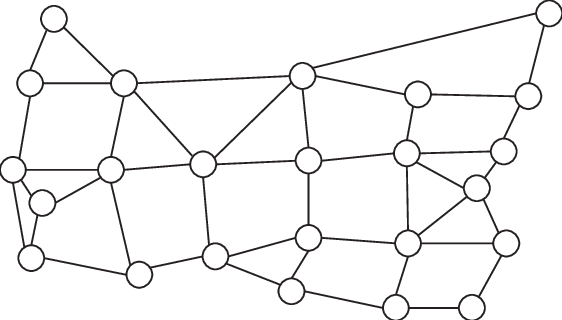
\includegraphics[scale=0.4]{images/usnet.png}
    \end{center}
\end{frame}
%-------------------------------------------------------------------------------
\begin{frame}{محیط ارزیابی}
    \begin{itemize}\RTList{}
        \item برای ارزیابی از زنجیره‌های تصادفی استفاده می‌شود و هر نمونه از ارزیابی میانگین ۱۰ اجرا می‌باشد.
        \item 
        زنجیره‌های تولید شده دارای گره‌ی آغازی و پایانی می‌باشند
        و ترافیک عبوری از آن‌ها ۲۵۰ واحد است.
    \end{itemize}
\end{frame}
%-------------------------------------------------------------------------------
\begin{frame}{شکاف بهینه الگوریتم بهینه}
    \begin{center}
        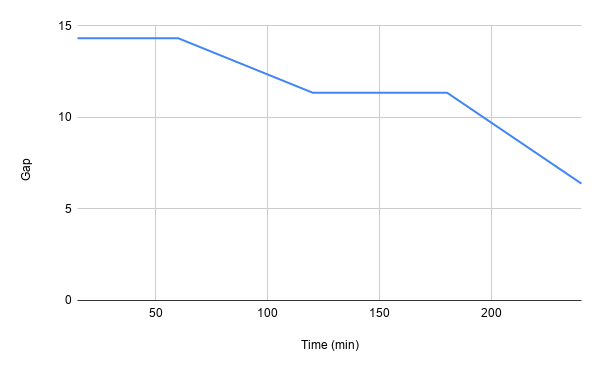
\includegraphics[scale=0.5]{images/chart-5.png}
    \end{center}
\end{frame}
%-------------------------------------------------------------------------------
\begin{frame}{نسبت سود به هزینه}
    \begin{center}
        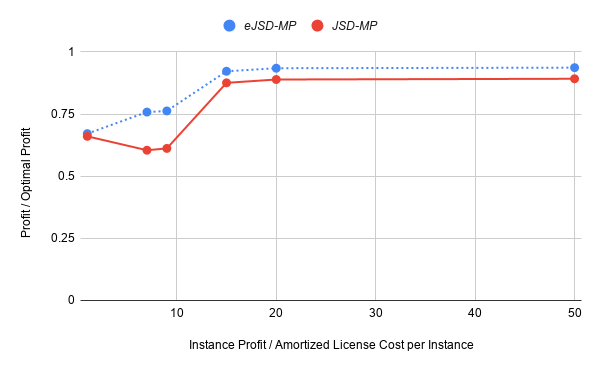
\includegraphics[scale=0.5]{images/chart-1.png}
    \end{center}
\end{frame}
%-------------------------------------------------------------------------------
\begin{frame}{سود نهایی در توپولوژی \lr{FatTree}}
    \begin{center}
        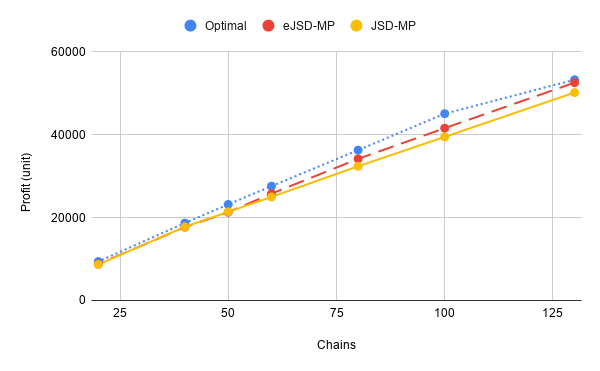
\includegraphics[scale=0.5]{images/chart-2.png}
    \end{center}
\end{frame}
%-------------------------------------------------------------------------------
\begin{frame}{سود نهایی در توپولوژی \lr{USnet}}
    \begin{center}
        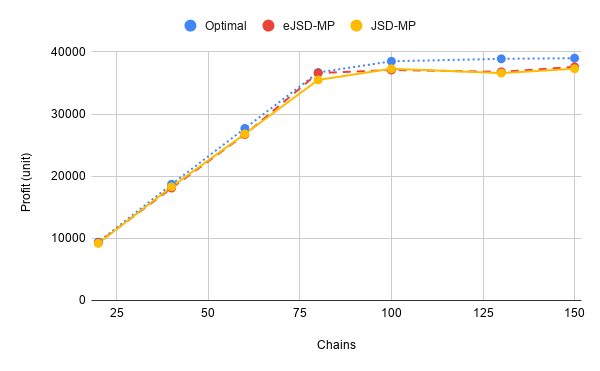
\includegraphics[scale=0.5]{images/chart-6.png}
    \end{center}
\end{frame}
%-------------------------------------------------------------------------------
\begin{frame}{جمع‌بندی}
    \begin{itemize}\RTList{}
        \item هر دو الگوریتم ارائه شده سود نهایی نزدیکی به الگوریتم بهینه ارائه می‌کنند.
        \item الگوریتم \lr{eJSD-MP} در زمان کمتر نتایجی بهتر یا برابر با الگوریثتم \lr{JSD-MP} ارائه می‌کند.
    \end{itemize}
\end{frame}
%-------------------------------------------------------------------------------
\begin{frame}[shrink=25]{مراجع}
    \begin{latin}
        \printbibliography[heading=none]
    \end{latin}
\end{frame}
%-------------------------------------------------------------------------------
% These are the hidden slides for giving more information
%-------------------------------------------------------------------------------
\begin{frame}{فرمول‌بندی}
    \par پارامترهای مساله
    \begin{center}\begin{latin}\begin{tabular}{|c|p{5cm}|}
        \hline
        \(memory(k)\) & required RAM of VNF instance with type \(k\) in GB \\
        \hline
        \(core(k)\) & required CPU cores of VNF instance with type \(k\) \\
        \hline
        \(\hat{memory}\) & required RAM of VNFM in GB \\
        \hline
        \(\hat{core}\) & required CPU cores of VNFM \\
        \hline
        \(capacity\) & maximum number of VNF instances that VNFM can handle \\
        \hline
        \(len(h)\) & number of VNF instances in \(h\)th SFC request \\
        \hline
    \end{tabular}\end{latin}\end{center}
\end{frame}
%-------------------------------------------------------------------------------
\begin{frame}{فرمول‌بندی}
    \par پارامترهای مساله
    \begin{center}\begin{latin}\begin{tabular}{|c|p{5cm}|}
        \hline
        \(type(v, k)\) & assuming the value 1 if the VNF instance \(v\) has type \(k\)  \\
        \hline
        \(bandwidth(u, v)\) & required bandwidth in link from VNF instance \(u\) to \(v\) \\
        \hline
        \(\hat{bandwidth}\) & required bandwidth in managmeent link \\
        \hline
        \(radius\) & maximum neighborhood distance for instance management \\
        \hline
    \end{tabular}\end{latin}\end{center}
\end{frame}
%-------------------------------------------------------------------------------
\begin{frame}{فرمول‌بندی}
    \par پارامترهای مساله
    \begin{center}\begin{latin}\begin{tabular}{|c|p{5cm}|}
        \hline
        \(licenseFee\) & VNFM license fee that must pay for each VNFM \\
        \hline
        \(vnfSupport(w)\) & assuming the value 1 if the physical server \(w\) can support VNF instances \\
        \hline
        \(isManageable(k)\) & assuming the value 1 if the type \(k\) needs a manager \\
        \hline
        \(notManagableBy(w1, w2)\) & assuming the value 1 if the physical server \(w1\) cannot manage by physical server \(w2\) \\
        \hline
    \end{tabular}\end{latin}\end{center}
\end{frame}
%-------------------------------------------------------------------------------
\begin{frame}{فرمول‌بندی}
    \par
    متغیرهای تصمیم‌گیری
    \begin{latin}\begin{tabular}{c p{10cm}}
        $x_h$ & binary variable assuming the value 1 if the $h$th SFC request is accepted; otherwise its value is zero \\
        $y_{wk}$ & the number of VNF instances of type $k$ that are used in server $w \in V_s^{PN}$ \\
        $z^k_{vw}$ & binary variable assuming the value 1 if the VNF node $v \in \cup_{i=1}^{T} V_{i, F}^{SFC}$ is served by the VNF instance of type k in the server $w \in V_s^{PN}$ \\
    \end{tabular}\end{latin}
\end{frame}
%-------------------------------------------------------------------------------
\begin{frame}{فرمول‌بندی}
    \par
    متغیرهای تصمیم‌گیری
    \begin{latin}\begin{tabular}{c p{10cm}}
        $\bar{y}_w$ & the number of VNFMs that are used in server $w \in V_s^{PN}$\\
        $\bar{z}_{hw}$ & binary variable assuming the value 1 if $h$th SFC is assigned to VNFM on server $w \in V_s^{PN}$\\
    \end{tabular}\end{latin}
\end{frame}
%-------------------------------------------------------------------------------
\begin{frame}{فرمول‌بندی}
    \par
    متغیرهای تصمیم‌گیری
    \begin{latin}\begin{tabular}{c p{10cm}}
        $\tau^{(u,v)}_{ij}$ & binary variable assuming the value 1 if the virual link $(u,v)$ is routed on the physical network link $(i,j)$\\
        $\bar{\tau}^{v}_{ij}$ & binary variable assuming the value 1 if the management traffic of VNF node $v$ is routed on the physical network link $(i,j)$\\
    \end{tabular}\end{latin}
\end{frame}
%-------------------------------------------------------------------------------
\end{persian}
\end{document}
